% ==============================================================================
\section{Synchronisation}

\label{SynchronisationTechnique}

% À charge à Bien Aimé et Ravi de remplir cette partie
% Indications :
%  Configuration des priorités etc.
%  Mode connecté (lié au serveur local)
%  Mode non connecté (à la Git-attitude)...
% 
% Bon courage ;-)

% ------------------------------------------------------------------------------
\subsection{Introduction}
L'objectif de cette section est de décrire les méthodes proposées afin de répondre au problème de synchronisation. Les échanges de données pouvant être limités (pas de réseau, liaison satellitaire uniquement) il convient de pouvoir choisir précisément les éléments que l'on souhaite synchroniser\footnote{Il est à noter que la synchronisation est bi-directionnelle : on reçoit les informations du serveur autant qu'on en envoie.}.\\
Pour permettre la gestion de ces éléments, on introduit la notion de \emph{priorité}; à chaque catégorie d'éléments (e.g. planning des transports, liste des fournisseurs, informations sur les véhicules, ...) peut être associée une priorité de laquelle dépendra la synchronisation ou non. À partir de cette \og{}hiérarchie d'importance\fg{}, on associe des \emph{profils de synchronisation} paramétrables qui - une fois activés - gère la synchronisation de façon transparente en fonction des choix de l'utilisateur.\\
Pour résoudre les problèmes de connexion et assurer le fonctionnement de la suite logicielle indépendamment de la liaison réseau, deux modes sont prévus :
\begin{itemize}
    \item Connecté
    \item Hors-ligne
\end{itemize}
L'utilisation de ces deux modes est décrit dans la Fig. \ref{explicationcodeco} : on utilise le mode connecté lorsque la liaison réseau est établie avec le serveur local; et le mode hors-ligne quand il n'y a pas de liaison avec le serveur local. Dans les deux cas, nous faisons abstraction de la liaison entre le serveur local et le serveur central dans la mesure où l'utilisateur ne se synchronisera qu'avec le serveur local.
% Schéma pour montrer la différence d'utilisation entre le mode connecté et hors ligne :
\begin{figure}[htbp]
    \centering
	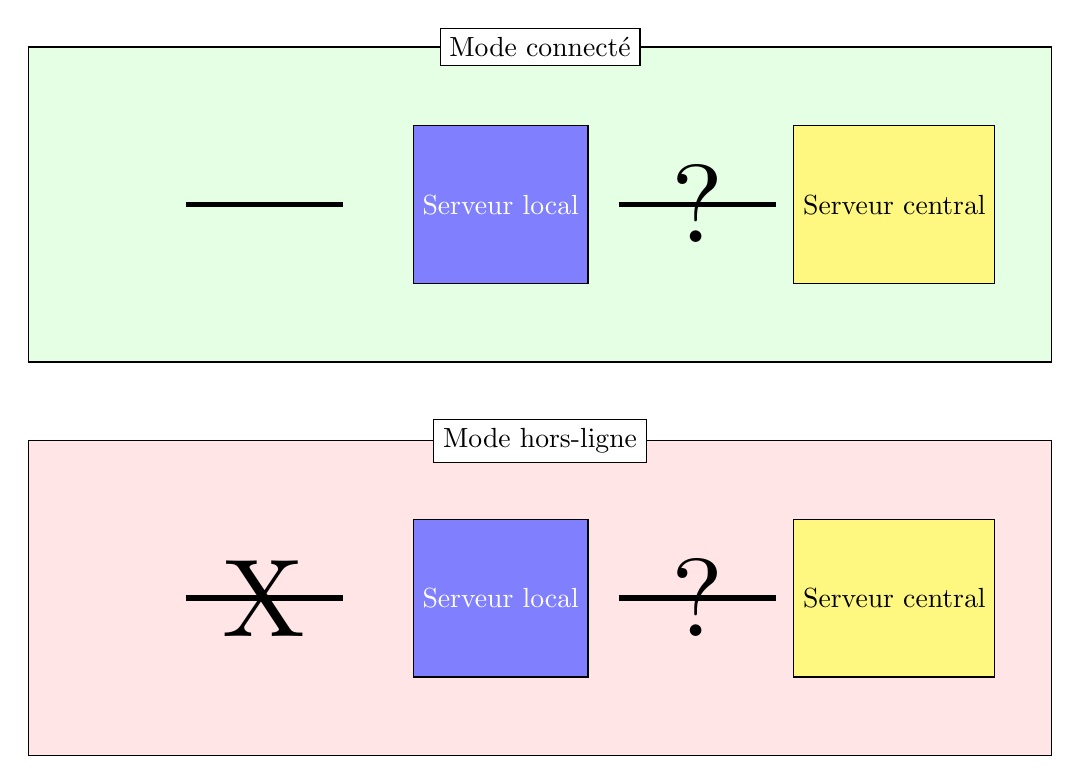
\begin{tikzpicture}
	    % Styles :
		\tikzstyle{titre}=[rectangle,draw,fill=white,text=black]
		\tikzstyle{symbole}=[rectangle,text=black, scale=4]
		\tikzstyle{serveurloc}=[rectangle,draw,fill=blue!50,text=white, minimum height=2cm]
		\tikzstyle{serveurcen}=[rectangle,draw,fill=yellow!50,text=black, minimum height=2cm]
	    % #### CADRE ROUGE :
		% Fond :
		\draw[fill=red!10] (0,0) rectangle (13, 4);
		% Titres :
		\node[titre] at (6.50,4.00) {Mode hors-ligne};
		% Serveurs :
		\node[serveurloc] at (6.00,2) {Serveur local};
		\node[serveurcen] at (11.00,2) {Serveur central};
		\node[symbole] at (8.50,2) {?};
		\node[symbole] at (3.00,2) {X};
		% Traits :
		\draw[line width=2pt] (2, 2) -- (4, 2);
		\draw[line width=2pt] (7.5, 2) -- (9.5, 2);
		% Utilisateurs :
		\umlactor[x=1.00, y=2]{Utilisateur}
		% #### CADRE VERT :
		% Fond :
		\draw[fill=green!10] (0,5) rectangle (13, 9);
		% Titres :
		\node[titre] at (6.50,9.00) {Mode connecté};
		% Serveurs :
		\node[serveurloc] at (6.00,7) {Serveur local};
		\node[serveurcen] at (11.00,7) {Serveur central};
		\node[symbole] at (8.50, 7) {?};
		% Traits :
		\draw[line width=2pt] (2, 7) -- (4, 7);
		\draw[line width=2pt] (7.5, 7) -- (9.5, 7);
		% Utilisateurs :
		\umlactor[x=1.00, y=7]{Utilisateur}
	\end{tikzpicture}
	\caption{Utilisation des modes connecté et hors-ligne}
	\label{explicationcodeco}
\end{figure}
    % TODO Schéma mode connecté
    % TODO Schéma mode hors-ligne
% Fin de la sous-section [Introduction]
% ------------------------------------------------------------------------------

% ------------------------------------------------------------------------------
\subsection{Gestion des priorités \& des profils de synchronisation}
Une priorité permettra à l'application de \og{}choisir\fg{} ce qui transitera sur le réseau. Cinq priorités seront définies (par ordre d'importance croissant) pour qualifier des éléments synchronisables :
\begin{enumerate}
    \item Négligeable
    \item Secondaire
    \item Normal
    \item Important
    \item Crucial
\end{enumerate}
L'utilisateur pourra gérer les priorités à synchroniser en les associant à un profil : lorsque l'utilisateur choisit un profil de synchronisation, seuls les éléments ayant une priorité inclue dans le profil sont synchronisés.
% Diagramme des CU pour la gestion des profils et des priorités :
\begin{figure}[htbp]
    \centering
	\begin{tikzpicture}
		\begin{umlsystem}[x=8.00,y=5.00,fill=yellow!10]{Priorités des éléments synchronisables}
			\umlusecase[x=0.00,y=1.00,name=MPrio]{Modifier la priorité d'un élément}
		\end{umlsystem}
		\begin{umlsystem}[x=8.00,y=0.00,fill=blue!10]{Profils de synchronisation}
			\umlusecase[x=0.00,y=0.00,name=ChProf]{Choisir un profil}
			\umlusecase[x=0.00,y=1.00,name=EProf]{Éditer un profil}
			\umlusecase[x=0.00,y=2.00,name=CrProf]{Creer un profil}
			\umlusecase[x=0.00,y=3.00,name=SProf]{Supprimer un profil}
		\end{umlsystem}
		\umlactor[x=0.00,y=3.00]{Utilisateur}
		\umlassoc{Utilisateur}{MPrio}
		\umlassoc{Utilisateur}{ChProf}
		\umlassoc{Utilisateur}{EProf}
		\umlassoc{Utilisateur}{CrProf}
		\umlassoc{Utilisateur}{SProf}
	\end{tikzpicture}
	\caption{Diagramme des cas d'utilisation pour la synchronisation}
	\label{ucsynchro}
\end{figure}
% Fin de la sous-section [Gestion des priorités]
% ------------------------------------------------------------------------------

% ------------------------------------------------------------------------------
\subsection{Mode connecté}
Dans ce mode, on suppose qu'il y a une liaison réseau entre l'utilisateur et le serveur local; toutes les modifications sont effectuées en \og{}temps réel\footnote{Un écart de temps pourra être constaté dans le cas où le réseau n'offre qu'un faible débit.}\fg{}. Pour ce mode, l'utilisateur doit :
\begin{enumerate}
    \item Se connecter
    \item Utiliser la suite logicielle
    \item Se déconnecter après utilisation
\end{enumerate}
L'utilisateur ne pourra effectuer que les modifications dont il a les \emph{permissions}.
% Diagramme des CU pour le mode connecté :
\begin{figure}[htbp]
    \centering
	\begin{tikzpicture}
		\begin{umlsystem}[x=5.00,y=0.00,fill=green!10]{Mode connecté}
			\umlusecase[x=1.00,y=1.50,name=Co]{Se connecter}
			\umlusecase[x=0.00,y=3.00,name=Modif, width=2cm]{Effectuer des modifications}
			\umlusecase[x=6.00,y=1.50,name=ChMode, width=2cm]{Choisir le mode connecté}
			\umlusecase[x=0.00,y=0.00,name=Deco]{Se déconnecter}
		\end{umlsystem}
		\umlactor[x=1.00,y=1.00]{Utilisateur}
		\umlinclude{Co}{ChMode}
		\umlinclude{Deco}{Co} 
		\umlinclude{Modif}{Co} 
		\umlassoc{Utilisateur}{Co}
		\umlassoc{Utilisateur}{Modif}
		\umlassoc{Utilisateur}{Deco}
	\end{tikzpicture}
	\caption{Diagramme des cas d'utilisation pour le mode connecté}
	\label{ucmodeco}
\end{figure}
% Fin de la sous-section [Mode connecté]
% ------------------------------------------------------------------------------

% ------------------------------------------------------------------------------
\subsection{Mode hors-ligne}
Contrairement au mode conecté, le mode hors ligne permet à l'utilisateur de modifier toutes les informations dont il dospose localement. Lorsqu'il souhaitera synchroniser ses informations avec le serveur, il devra se connecter et c'est à ce moment là que le serveur vérifiera que l'utilisateur n'outrepasse pas les droits qui lui sont accordés. Si c'est le cas, le serveur rejettera les modifications locales.
% Diagramme des CU pour le mode hors ligne :
\begin{figure}[htbp]
    \centering
	\begin{tikzpicture}
		\begin{umlsystem}[x=5.00,y=0.00,fill=red!10]{Mode hors-ligne}
			\umlusecase[x=4.50,y=0.20,name=Co]{Se connecter}
			\umlusecase[x=0.00,y=3.00,name=Modif, width=2cm]{Effectuer des modifications}
			\umlusecase[x=6.00,y=3.00,name=ChMode, width=2cm]{Choisir le mode hors-ligne}
			\umlusecase[x=0.00,y=1.00,name=Sync, width=2cm]{Synchroniser avec le serveur}
		\end{umlsystem}
		\umlactor[x=1.00,y=1.00]{Utilisateur}
		\umlinclude{Co}{ChMode}
		\umlinclude{Sync}{Co} 
		\umlassoc{Utilisateur}{Modif}
		\umlassoc{Utilisateur}{Sync}
	\end{tikzpicture}
	\caption{Diagramme des cas d'utilisation pour le mode hors-ligne}
	\label{ucmodedeco}
\end{figure}
% Fin de la sous-section [Mode hors-ligne]
% ------------------------------------------------------------------------------

% ------------------------------------------------------------------------------
\subsection{Gestion des conflits}
Durant la synchronisation, que ce soit en mode connecté ou hors-ligne, des conflits peuvent survenir au niveau du contenu des informations. Dans ce cas, l'utilisateur est averti du conflit et des informations qu'il touche et il lui revient le soin de les gérer en choisissant explicitement ce qui est correct et qui doit être enregistré sur le serveur.\\
Afin de savoir si la version des informations sur le serveur est plus récente (ou plus vieille) que la version locale, un horodatage est mis en place tel que :
\begin{itemize}
    \item Chaque modification locale est horodatée avec l'heure locale
    \item À la synchronisation, l'écart temporel entre l'heure locale et l'heure serveur est mesuré\footnote{Par exemple, supposons que la machine locale retarde de deux heures : si une information a été modifiée à 17h (heure serveur) et qu'une modification est apportée à 16h le même jour en local, l'écart de deux heures entre les deux machines est mesuré lors de la synchronisation (i.e. deux heures) et permet de dater réellement la modification en local et ainsi déterminer laquelle succède à l'autre. À cette fin, l'application enregistre les éventuels changements d'heure oppérés en local pour notifier le serveur des écarts d'horodatage.}
\end{itemize}
% Fin de la sous-section [Gestin des conflits]
% ------------------------------------------------------------------------------

% Fin de la section [Synchronisation]
% ==============================================================================
